\chapter{Mathematical Derivations}
\label{sec:proofs}


\section{Simplified equations of motion for diagonal $R$}
\label{sec:Rdiagndof}

Here the derivation of the simplified form of equations of motion, where intrinsic and extrinsic forces are two separate terms, is derived for a class of $n$-DoF fully actuated robots.

\subsection{Assumptions} 

Three assumptions are necessary for this form. First, the robotic system is fully-actuated, i.e. $m=n$, so that the matrix $R$ is square and invertible. Second, that a coordinates system can be selected so that the gear-ratio matrix $R$ is diagonal for all possible configurations:
%
\begin{align}
R_{i,j} = 0 \quad \forall \; i \neq j
\end{align}
%
Third, that dynamic forces related to viscous damping and inertial forces in motor rotor are linear with respect to rotor velocity:
%
\begin{align}
\vec{\tau}_{rotor-inertia} = I \dot{\vec{w}}  \quad  \vec{\tau}_{rotor-damping} = B \vec{w}
\end{align}
%
where  matrices $I$ and $D$ are diagonal since motor rotors are not coupled directly. 

\subsection{Derivation}

Starting from the general eq.\eqref{eq:eom_ndof} the EoM are:
%
\begin{align}
H \vec{ \ddot{q} } + C\vec{ \dot{q} } + D \vec{ \dot{q} } + \vec{ g }
		= R^T  \left[ 
		\vec{ \tau } - I \vec{ \dot{w} } - B \vec{ w }       
		\right]
\end{align}
%
Then substituting motor velocities with joint coordinates, using the kinematic relation of eq. \eqref{eq:coortransform}:
%
\begin{align}
H \vec{ \ddot{q} } + C\vec{ \dot{q} } + D \vec{ \dot{q} } + \vec{ g }
		&= R^T  \left[ 
		\vec{ \tau } - I R \vec{ \ddot{q} } - B R\vec{ \dot{q} }       
		\right] \\
H \vec{ \ddot{q} } + C\vec{ \dot{q} } + D \vec{ \dot{q} } + \vec{ g }
		&= R^T \vec{ \tau } - R^T I R \vec{ \ddot{q} } - R^T B R \vec{ \dot{q} }  
\end{align}
%
Then because $R$, $I$ and $B$ matrix are diagonal, they can be permuted and also $R^T=R$. Hence, the EoM can be rearranged:
%
\begin{align}
H \vec{ \ddot{q} } + C\vec{ \dot{q} } + D \vec{ \dot{q} } + \vec{ g }
		&= R \vec{ \tau } - R R I \vec{ \ddot{q} } - R R B \vec{ \dot{q} }  
\end{align}
%
Then, assuming the robotic system is fully actuated, the R matrix is square and invertible. Then multiplying by $R^{-1}$ from the left on both side:
%
\begin{align}
R^{-1} \left[ H \vec{ \ddot{q} } + C\vec{ \dot{q} } + D \vec{ \dot{q} } + \vec{ g } \right]
		&= \vec{ \tau } - R I \vec{ \ddot{q} } - R B \vec{ \dot{q} }  
\end{align}
%
Then rearranging:
%
\begin{align}
R^{-1} \left[ H \vec{ \ddot{q} } + C\vec{ \dot{q} } + D \vec{ \dot{q} } + \vec{ g } \right]
		&= \vec{ \tau } - R  \left[ I \vec{ \ddot{q} } + B \vec{ \dot{q} }  \right]
\end{align}
%
and thus obtain the desired final form:
%
\begin{align}
\vec{ \tau } &=  R^{-1} \underbrace{ \left[ H \vec{ \ddot{q} } + C\vec{ \dot{q} } + D \vec{ \dot{q} } + \vec{ g } \right] }_{\vec{\tau}_E}
 + R \underbrace{ \left[ I \vec{ \ddot{q} } + B \vec{ \dot{q} }  \right]}_{\vec{\tau}_I}
\end{align}
%



\newpage
\section{Optimal gear-ratio along a known trajectory}
\label{sec:optgearproof}

Assuming that the robot is fully actuated and viscous forces linear in speed, it is possible to derive closed form expression for the optimal gear-ratios on a known trajectory.


\subsection{Single DoF}
\label{sec:optgearproof1}

Starting with the EoM in inverse dynamic form (from eq. \eqref{eq:1dofEoM}):
%
\begin{align}
\tau  &=  \frac{\tau_E}{R} + R \tau_I
\end{align}
%
Using a quadratic cost function to minimize:
%
\begin{align}
J &=  \tau^2 = \frac{\tau_E^2}{R^2} + 2 \tau_E \tau_I + R^2 \tau_I^2
\label{eq:Jonedof}
\end{align}
%

Finding the gear-ratio that minimizes this cost can be formulated as:
%
\begin{align}
R^* &=  \operatornamewithlimits{argmin}\limits_{R} J \\
   &   \text{s.t.} \quad R \in \Re  \quad \& \quad R > 0
\end{align}
%
A non-real value would have no physical sense. A negative $R$ value would be physically possible, for instance the reverse gear in a car. However, for symmetric electric motors, in the sense that they behave the same way for any sign of torque and speed, there should be no gain obtained by changing the direction of the motor velocity. This is consistent with cost function which is symmetric with respect to $R$:
%
\begin{align}
J(R) = J( -R )
\end{align}
%

\paragraph{Derivation}

First finding the partial derivative of the cost $J$ with respect to $R$:
%
\begin{align}
\frac{ \partial J }{ \partial R  } &=  2 \tau \frac{ \partial \tau }{ \partial R } = 2 \left( \frac{\tau_E}{R} + R \tau_I \right) \left( -\frac{\tau_E}{R^2} + \tau_I \right) \\
\frac{ \partial J }{ \partial R  } &= 2 \left( R \tau_I^2 - \frac{\tau_E^2}{R^3} \right)
\end{align}
%
Then the second derivative:
%
\begin{align}
\frac{ \partial^2 J }{ \partial R^2  } &= 2 \left( \tau_I^2 + 3 \frac{\tau_E^2}{R^4} \right)
\end{align}
%
Hence, on the domain of interest, the second derivative is always positive:
%
\begin{align}
\frac{ \partial^2 J }{ \partial R^2  } \geq 0  \quad \forall \quad R \in (0,+\infty)
\end{align}
%
Thus the cost function $J$ is convex on the desired interval of possible $R$ values. The minimum of the function can thus be found by solving for the point where the first derivative is equal to zero:
%
\begin{align}
0 &= \frac{ \partial J }{ \partial R  } = 2 \left( R \tau_I^2 - \frac{\tau_E^2}{R^3} \right) \\
R \tau_I^2 &= \frac{\tau_E^2}{R^3} 
\end{align}
%
Since $R>0$, it is possible to multiply both side by $R^3$, leading to
%
\begin{align}
R^4 \tau_I^2 &= \tau_E^2
\end{align}
%
Then, assuming a non-degenerative case of $\tau_I \neq 0$, it leads to
%
\begin{align}
R^4  &= \frac{\tau_E^2}{\tau_I^2} \\
R^2  &= \pm \sqrt{ \frac{\tau_E^2}{\tau_I^2} } = \pm \frac{\tau_E}{\tau_I} \\
R    &= \pm \sqrt{ \pm \frac{\tau_E}{\tau_I} } 
\end{align}
%
Then, the only real and positive solution to this equation is given by:
%
\begin{align}
R    &= \sqrt{ \left| \frac{\tau_E}{\tau_I} \right|} 
\end{align}
%

\paragraph{Solution}

The minimal cost value is thus obtain with the optimal gear-ratio value:
%
\begin{align}
R^*    &=  \operatornamewithlimits{argmin}\limits_{ R > 0 } J = \sqrt{ \left| \frac{\tau_E}{\tau_I} \right|} 
\end{align}
%
Which lead to the minimum cost:
%
\begin{align}
J^*    &=  2 \tau_E \tau_I  + 2 \left| \tau_E \tau_I \right| 
\end{align}
%
Note that the the minimized cost is zero when extrinsic and intrinsic forces have opposite signs.

\paragraph{Degenerative cases}
Here degenerative situations when the intrinsic forces or extrinsic forces are equal to zero are investigated, based on \eqref{eq:Jonedof}.
%
If the intrinsic forces are equal to zero, then the cost tends towards zero as the gear-ratio $R$ tends toward $\infty$:
%
\begin{align}
\tau_I = 0 \quad \& \quad R \rightarrow \infty \quad \Rightarrow \quad J \rightarrow 0
\end{align}
%
If the extrinsic forces are equal to zero, then the cost tends towards zero as the gear-ratio $R$ tends toward zero:
%
\begin{align}
\tau_E = 0 \quad \& \quad R \rightarrow 0 \quad \Rightarrow \quad J \rightarrow 0
\end{align}
%
If both the extrinsic forces and intrinsic forces are equal to zero, then the cost is zero for any gear-ratio:
%
\begin{align}
\tau_E = 0 \quad \& \quad \tau_I = 0 \quad \Rightarrow \quad J = 0  \quad \forall R
\end{align}
%

%%%%%%%%%%%%%%%%%%%%%%%%%%%%%

\subsection{Multiple DoF}
\label{sec:optgearproofn}

Starting with the EoM in inverse dynamic form (from eq. \eqref{eq:eom_ndof2}):
%
\begin{align}
\vec{ \tau } &=  R^{-1} \vec{\tau}_E + R \vec{\tau}_I
\end{align}
%
Using the following quadratic cost function:
%
\begin{align}
J &=  \vec{ \tau }^T \vec{ \tau }
\end{align}
%
Finding the gear-ratios matrix $R$ that minimize this cost can be formulated as
%
\begin{align}
R^* &=  \operatornamewithlimits{argmin}\limits_{R} J \\
    &   \text{s.t.} \quad R_{i,j} \in \Re  \quad \& \quad R_{i,j} > 0  
\end{align}
%

An analytic solution is available if the gear-ratios matrix $R$ is diagonal.

\paragraph{Derivation}

Using index notation, the EoM and cost function can be written as:
%
\begin{align}
\vec{ \tau } =  R^{-1} \vec{\tau}_E + R \vec{\tau}_I \quad &\Rightarrow \quad \tau_i = \sum_j{ \left[ R^{-1}\right]_{i,j} \tau_j^E + R_{i,j} \tau_j^I }\\
J =  \vec{ \tau }^T \vec{ \tau } \quad &\Rightarrow \quad J = \sum_i{ \tau_i^2 }
\end{align}
%
Note that here, superscript instead of subscript are used to identify extrinsic and intrinsic forces, to avoid confusion with indexes. Then the properties due to the diagonality of matrix $R$ can be used:
%
\begin{align}
R_{i,j}                    &= 0 \quad \forall \quad i \neq j \\
\left[ R^{-1}\right]_{i,j} &= 0 \quad \forall \quad i \neq j \\
\left[ R^{-1}\right]_{i,i} &= \left( R_{i,i}  \right)^{-1}
\end{align}
%
Then the equations can be simplified to:
%
\begin{align}
\tau_i &= \left( R_{i,i}  \right)^{-1} \tau_i^E + R_{i,i} \tau_i^I \\
J      &= \sum_i{ \left[  \left( R_{i,i}  \right)^{-1} \tau_i^E + R_{i,i} \tau_i^I   \right]^2 }
\end{align}
%
By inspection, it is possible to see that the cost $J$ is the sum of $n$ independent terms (one per DoF), and that given the assumptions those terms are independent. Hence, the cost $J$ can be minimized by minimizing individually each term with the appropriate $R_{i,i}$. The solution for minimizing each of those term is identical to the one for a single DoF robot, see section \ref{sec:optgearproof1}. Leading to 
%
\begin{align}
R_{i,i}^* = \sqrt{\left| \frac{\tau_i^E}{\tau_i^I}\right|}
\end{align}
%

\paragraph{Solution}
The optimal gear-ratio matrix, is thus constructed from independent solutions on each DoF:
%
\begin{align}
R^* = \left \{
\begin{array}[pos]{l}
	R^*_{i,j} = \sqrt{\left| \frac{\tau_i^E}{\tau_i^I}\right|} \quad \forall \quad i = j \\
	R^*_{i,j} = 0                                              \quad \forall \quad i \neq j
\end{array} \right.
\end{align}
%
Leading to the following total minimum cost:
%
\begin{align}
J^*   &= 2 \sum_i{ \left[ \tau_i^E \tau_i^I + \left| \tau_i^E \tau_i^I \right| \right] }
\end{align}
%

\newpage
\section{Stability Proofs}
\label{sec:stabproofs}

 
\subsection{R* Computed Torque Controller}
\label{sec:stabrstar1}

In this section, the stability of motions when using the R* Computed Torque Controller is demonstrated for any arbitrary sequence of selected gear-ratio. However, here perfect knowledge of the equation of motions is assumed.

The equation of motions can take this simple but general form:
\begin{align}
H_k \ddot{\vec{q}} + \vec{c}_k = R_k \vec{\tau} \quad \forall k \in \{1,...,l\}
\label{eq:eom_k}
\end{align}
where subscript $k$ is used to emphasized the dependence to the discrete gear-ratio selection. The total inertia matrix $H_k$ and state-dependent forces $c_k$ are given by:
\begin{align}
H_k       &= H(\vec{q}) + R_k^T I R_k \\
\vec{c}_k &= \left( D + R_k^T B R_k \right) \dot{\vec{q}} + C( \dot{\vec{q}} , \vec{q} ) \dot{\vec{q}} + \vec{g}(\vec{q})
\end{align}
In the computed torque scheme, it is assumed that based on state measurement those term can be computed exactly. In addition here, it is assumed the controller is also aware of the discrete gear-ratio state $k$.

The control law for motor torques takes the following form:
\begin{align}
\vec{\tau} = R_k^{-1} \left( H_k \ddot{\vec{q}}_r + \vec{c}_k \right) 
\label{eq:ctc_k}
\end{align}
where the vector $\ddot{\vec{q}}_r$ represents instantaneous desired acceleration. The control law for the gear-ratio selection takes the form of an optimization, however here stability is demonstrated for the more general case of arbitrary gear-ratio sequence. Hence the stability result can be extended for any type of gear-ratio selection scheme used in conjunction with the computed torque. 

When substituting the control law, eq.\eqref{eq:ctc_k}, in the equations of motion, eq.\eqref{eq:eom_k}, then the resulting closed-loop behavior is simply:
\begin{align}
\ddot{\vec{q}} = \ddot{\vec{q}}_r \quad \forall k
\label{eq:cl_k}
\end{align}
Hence, the system is not only linear in behavior (form a $\ddot{\vec{q}}_r$ input point of view) but also continuous, non-linearities and discontinuities are compensated by computing the inverse dynamic of the system.

Specifying $\ddot{\vec{q}}_r$ based on state is equivalent to designing a controller for a linear second-order $n$-DoF system. For trajectory tracking the following proportional-derivative control laws can be used:
\begin{align}
\ddot{\vec{q}}_r &= \ddot{\vec{q}}_d + K_D ( \dot{\vec{q}}_d - \dot{\vec{q}} ) + K_P \underbrace{( \vec{q}_d - \vec{q} ) }_{\vec{q}_e}
\end{align}
leading to second order error dynamics:
\begin{align}
0 &= \ddot{\vec{q}}_e + K_D \dot{\vec{q}}_e + K_P \vec{q}_e
\end{align}
Hence, convergence of error to zero is guaranteed if both gain matrix $K_D$ and $K_P$ are positive definite:
\begin{align}
\vec{q}_e \rightarrow \vec{0} \quad\text{ with }\quad K_D > 0 \, , \, K_P > 0
\end{align}


%%%%%%%%%%%%%%%%%%%%%%%%%%%%%%%%%%%%%%%%%%%%

\newpage

\subsection{R* Sliding Mode Controller}
\label{sec:stabrstar2}

In this section, the stability of motions when using the R* Sliding Mode Controller is demonstrated for any arbitrary sequence of selected gear-ratio, in the presence of bounded uncertainty.

The equation of motions can take this simple but general form:
\begin{align}
H_k \ddot{\vec{q}} + \vec{c}_k = R_k \vec{\tau} + \vec{d} \quad \forall k \in \{1,...,l\}
\label{eq:eom_kd}
\end{align}
where $\vec{d}$ is an unknown generalized force vector that can represent disturbance or modeling errors.

The proposed control law for motor torques takes the form:
%
\begin{align}
\vec{\tau} = R_k^{-1} \left( H_k \ddot{\vec{q}}_r + \vec{c}_k - G_k sgn( \vec{s} ) \right) 
\label{eq:slidinglaw}
\end{align}
%
leading to the following closed-loop behavior:
%
\begin{align}
H_k ( \ddot{\vec{q}} - \ddot{\vec{q}}_r ) = \vec{d} - G_k sgn( \vec{s} ) \quad \forall k
\label{eq:slidinglawcl}
\end{align}
%
which has two types of discontinuities: 1) discontinuous torque term introduced by the sliding mode controller and 2) arbitrary selected gear-ratio $k$.
%
The following variables are then introduced:
%
\begin{align}
\vec{q}_e       &= \vec{q}_d       - \vec{q} \\
\dot{\vec{q}}_r &= \dot{\vec{q}}_d - \lambda  \vec{q}_e \\
\vec{s}         &= \dot{\vec{q}}_e + \lambda  \vec{q}_e  = \dot{\vec{q}} - \dot{\vec{q}}_r \\
\dot{\vec{s}}   &= \ddot{\vec{q}}_e + \lambda  \dot{\vec{q}}_e  = \ddot{\vec{q}} - \ddot{\vec{q}}_r
\end{align}
%
where lambda is a positive constant. Then convergence to the desired trajectory can be guaranteed if the sliding variables $\vec{s}$ converge to zero \cite{slotine_applied_1991}. The basic idea is that if a Lyapunov-like quadratic function of the sliding variable is only decreasing in time, then sliding variables will converge to zero, which also implies that the error will converge to zero:
%
\begin{align}
V = \vec{s}^T \vec{s} \rightarrow 0 \quad\Rightarrow\quad  \vec{s} \rightarrow \vec{0} \quad\Rightarrow\quad \vec{q}_e \rightarrow \vec{0}
\end{align}
%
Note that here the Lyapunov-like function must be continuous and the same for all discrete mode, and its derivative negative definite for all discrete modes $k$ for the argument to hold for arbitrary sequence of gear-ratio $k$ \cite{liberzon_switching_2003}:
%
\begin{align}
\dot{V}_k < 0 \quad \forall k \quad \quad\Rightarrow\quad V \rightarrow 0
\end{align}
%
One way to guarantee the sliding condition is individually for each DoF $i$ and each possible mode $k$:
%
\begin{align}
\frac{d( s_i^2 )}{dt} < -\eta |s_i| \; \quad \forall i \; \forall k
\label{eq:slidingcondition}
\end{align}
%
where $\eta$ is a small positive constant. From eq.\eqref{eq:slidinglawcl}, sliding variable derivative is given by:
%
\begin{align}
\dot{\vec{s}} = H_k^{-1}(\vec{d} - G_k sgn( \vec{s} ))
\end{align}
%
Substituting in the sliding condition equation leads to:
%
\begin{align}
s_i \dot{s}_i  = s_i \left( \left[ H_k^{-1} \vec{d} \right]_i - \left[ H_k^{-1} G_k sgn(\vec{s}) \right]_i \right) < -\eta |s_i|
\end{align}
%
If the matrix gain is parametrized in the following way:
%
\begin{align}
G_k = H_k K_k
\end{align}
%
where $K_k$ is a diagonal matrix. Then the discontinuous gain term is uncoupled in the sliding condition equation:
%
\begin{align}
s_i \left( \left[ H_k^{-1} \vec{d} \right]_i - K_{ii} sgn( s_i ) \right) &< -\eta |s_i| \\
 \left[ H_k^{-1} \vec{d} \right]_i s_i + \eta |s_i| &< K_{ii} | s_i | \\
 \eta  \pm  \left[ H_k^{-1} \vec{d} \right]_i &< K_{ii} 
\end{align}
%
which can be guaranteed if the gain are selected such that:
%
\begin{align}
K_{ii} = \operatornamewithlimits{max}\limits_{\vec{d}} \left[ H_k^{-1} \vec{d} \right]_i + \eta
\label{eq:slidinggain}
\end{align}
%
Thus, if the gains are defined based on disturbance bounds and according to eq.\eqref{eq:slidinggain}, the sliding condition is guaranteed for all gear-ratio mode $k$, and thus convergence to the desired trajectory is guaranteed for any gear-ratio sequence. Note that the gain $K_{ii}$ is a function of the discrete selected gear-ratio mode $k$. 


%%%%%%%%%%%%%%%%%%%%%%%%%%%%%%%%%%%%%%%%%%%%%%%%%%%%%%%%%%%%%%%%%%%%%%%%%%%%%%%%%%%%%%%%%%%%%%%%%%%%%%%%%5


\newpage

\section{Chattering Bounds with Rollout Gear-selection}
\label{sec:chat}

This section computes lower bounds for the time interval between successive gear-shifts when using the Rollout gear-selection scheme. 

\paragraph{Problem setting}
First, using the Rollout approach, the optimal gear-ratio mode $k^*$ selection is done as follow:
%
\begin{align}
k^*(t)   &= \operatornamewithlimits{argmin}\limits_{k} \left[ J_k(t) + Q \, [[ k \neq k_{previous}]] \, \right]
\label{eq:rolloutsimple}
\end{align}
%
where $J_k(t)$ is the computed cost over the simulated trajectory over the time horizon $h$ using the gear-ratio mode $k$. An additional instantaneous cost $Q$ is added when the gear-ratio mode is changed.
%
The integral cost is given by:
%
\begin{align}
J_k(t) = \int_{t}^{t+h}{  C_k( \hat{\vec{x}}_k ) \, d\hat{t} }
\end{align}
%
where $C_k$ is the instantaneous cost, $\hat{t}$ is the virtual time in the simulations and $\hat{\vec{x}}$ the predicted trajectory. The virtual state trajectory is computed by simulating the system in closed-loop, using the base-policy, and integrating forward starting from the actual state at time $t$:
%
\begin{align}
\hat{\vec{x}}_k( \hat{t} , t ) = \int_{t}^{\hat{t}}{  \dot{\hat{\vec{x}}}_k \, d\tilde{t} } + \vec{x}(t)
\end{align}
%
If both the real system and simulations are robustly staying on the desired trajectory, then the virtual states in the simulation are independent of actual starting simulation time:
%
\begin{align}
\hat{\vec{x}}_k( \hat{t} , t ) = \vec{x}( \hat{t} ) =  \vec{x}_d( \hat{t} )
\end{align}
%
In this thesis the instantaneous cost is usually taken to be squared actuator torques:
%
\begin{align}
C_k =  \vec{\tau}_k^T \vec{\tau}_k
\end{align}
%
where $\vec{\tau}_k$ is the computed torque in predictive simulation with the base policy when using the gear-ratio mode $k$.
%
It will be assumed that an upper bound can be found for the instantaneous cost, at least in a domain of interest $D$, given the desired trajectory and the feedback policy:
%
\begin{align}
C_k^{max} =  \operatornamewithlimits{max}\limits_{\vec{x},t \in D} C_k(\vec{x},t)
\end{align}
%
Such a bound should always exist given reasonable assumptions: 
\begin{itemize}
	\item Domain of interest $D$ constraint all states to finite values
	\item Desired trajectory has bounded acceleration, speed and position values 
	\item Absence of singularity where inertia matrix values can tend toward infinity
\end{itemize}

For instance, if using computed torque as base policy and a torque-squared criteria, the maximum instantaneous cost value is given by:
%
\begin{align}
C_k^{max} =  \operatornamewithlimits{max} \vec{\tau}_k^T \vec{\tau}_k \leq \sum \operatornamewithlimits{max} \left[\vec{\tau}_{k}\right]_{i}^2 
\end{align}
%
where $\operatornamewithlimits{max} \left[\vec{\tau}_{k}\right]_{i}$ is the maximum value that can be computed for joint $i$ when using the gear-ratio $k$.

\subsection{On a trajectory}
\label{sec:chat1}

Here a minimum time delay for a back-and-forth gear-shift sequence is derived for the situation where the robot has converged on a trajectory and is staying on the trajectory. In that case, it is assumed that both the simulation trajectory and the real system follow the same desired trajectory, see Fig. \ref{fig:costontrajrollout}.

\begin{figure}[H]
	\centering
		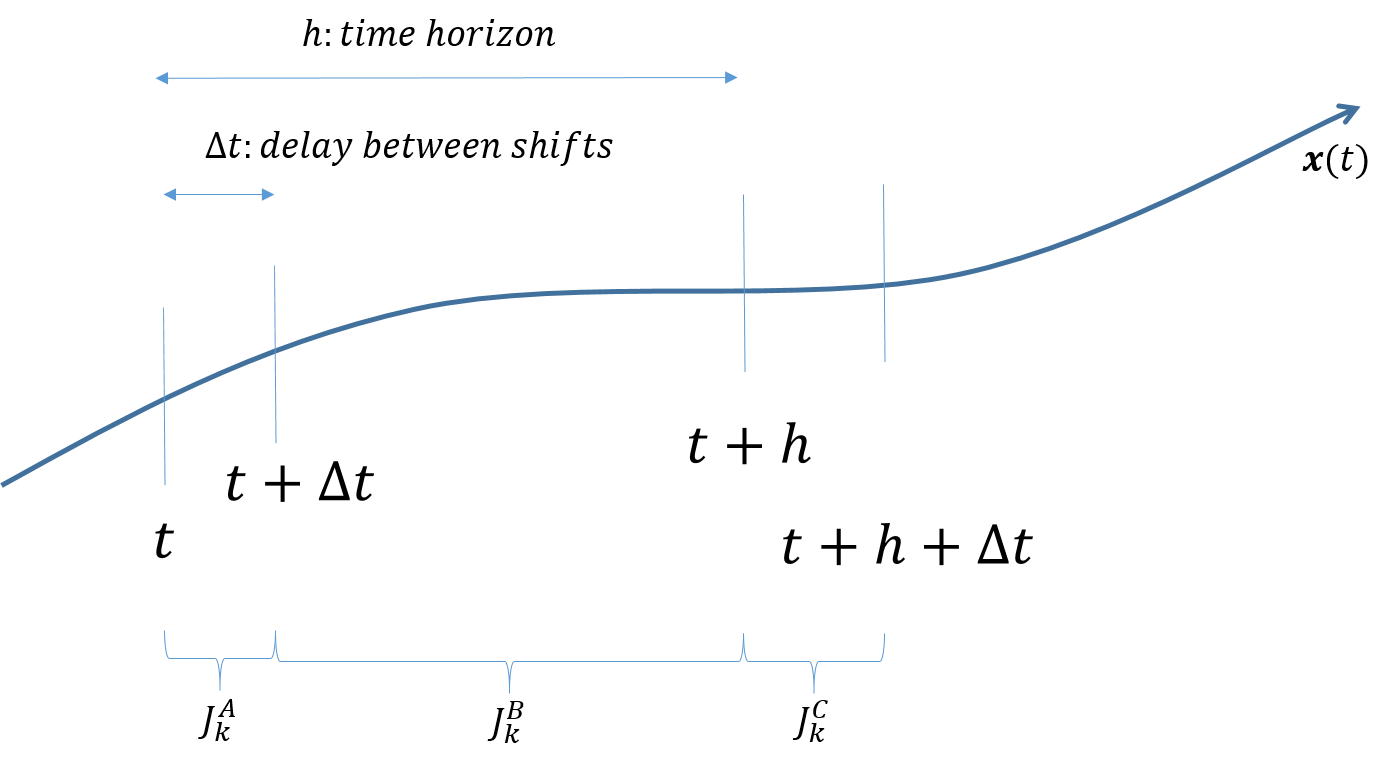
\includegraphics[width=0.90\textwidth]{costontrajrollout.png}
	\caption{Rollout controller behavior on a given trajectory}
	\label{fig:costontrajrollout}
\end{figure}

%It can be shown that there is a minimum delay $\Delta t$ between a back-and-forth gear-shift sequence. Hence, no arbitrary fast chattering between gear-ratio (zeno behavior \cite{liberzon_switching_2003}) is possible. 

\paragraph{Proof} 

Without loss of generality, lets assume a gear shift sequence where the robot is first using mode $i$, then shift to mode $j$ at time $t$ and then shift back to mode $i$ at time $t+\Delta t$. If such a sequence happened while using the gear-ratio selection law given by eq. \eqref{eq:rolloutsimple}, then the following inequality must have been satisfied:
%
\begin{align}
i \rightarrow j  \quad\text{at time}\quad t          &\quad\Rightarrow\quad J_j(t) + Q < J_i(t)                  \\
j \rightarrow i  \quad\text{at time}\quad t+\Delta t &\quad\Rightarrow\quad J_i(t+\Delta t) + Q < J_j(t+\Delta t)
\end{align}
%
Then to simplify the notation, integral cost on the trajectory is given by the following value for each three sections of interest:
%
\begin{align}
J_k^A = \int_{t}^{t+\Delta t}{         C_k  d\hat{t}  }   \quad \quad
J_k^B = \int_{t+\Delta t}^{t+h}{       C_k  d\hat{t}  }   \quad \quad
J_k^C = \int_{t+h}^{t+\Delta t+h}{     C_k  d\hat{t}  }
\end{align}
%
Then it is possible to express the computed cost of predictive simulation done at $\Delta t$ time difference by the sum of an identical part and a different part:
%
\begin{align}
J_k(t)          &= \int_{t}^{t+h}{ C_k   d\hat{t} }  = J_k^A + J_k^B \\
J_k(t+\Delta t) &= \int_{t+\Delta t}^{t+\Delta t+h}{   C_k  d\hat{t}} = J_k^B + J_k^C
\end{align}
%
The difference between computed costs separated by $\Delta t$ is:
%
\begin{align}
\Delta J_k = J_k(t+\Delta t) - J_k(t) &= J_k^C - J_k^A
\end{align}
%
Now assuming there is an upper bound on instantaneous cost $C_k^{max}$, an upper bound also exist integral costs over a finite amount of time. Since the instantaneous cost is always positive definite, the integral cost cannot be negative. Hence:
%
\begin{align}
0 \leq J_k^C   \leq  C_k^{max} \Delta t \\
0 \leq J_k^A   \leq  C_k^{max} \Delta t 
\end{align}
%
The cost variation is thus bounded is this range:
%
\begin{align}
-C_k^{max} \Delta t  \leq \Delta J_k \leq C_k^{max} \Delta t
\label{eq:costvariation}
\end{align}
%
Hence the time evolution of computed cost can be bounded:
%
\begin{align}
J_j(t+\Delta t) \leq J_j(t)  + C_k^{max} \Delta t \\
J_i(t+\Delta t) \geq J_i(t)  - C_k^{max} \Delta t 
\end{align}
%
Finally it is possible to combine all those inequality, starting with the condition for the second gearshift:
%
\begin{align}
J_i(t)  - C_k^{max} \Delta t + Q \leq J_i(t+\Delta t) + Q &< J_j(t+\Delta t) \leq J_j(t)  + C_k^{max} \Delta t \\
J_i(t) + Q &\leq J_j(t)  + 2 C_k^{max} \Delta t \\
J_j(t) + 2 Q &\leq J_j(t)  + 2 C_k^{max} \Delta t \\
Q &\leq C_k^{max} \Delta t 
\end{align}
%
Hence resulting in the desired inequality relating instantaneous cost and time between gear-shift:
%
\begin{align}
\Delta t \geq \frac{Q}{C_k^{max}}
\end{align}
%
Note that if there is more than 2 discrete gear-ratio options, this analysis gives not insight about possible sequences of gear-shift during this interval, but still guarantee the minimum time for a full cycle (coming back to the starting gear-ratio).







%%%%%%%%%%%%%%%%%%%%%%%%%%%%%%%%%%%%%%%
\subsection{Arbitrary}
\label{sec:chat2}

Fig. \ref{fig:rollouttrajs} gives a graphical support illustrating the 2D space, where at all time virtual trajectories branch-off the real robot trajectory.
%
\begin{figure}[H]
	\centering
		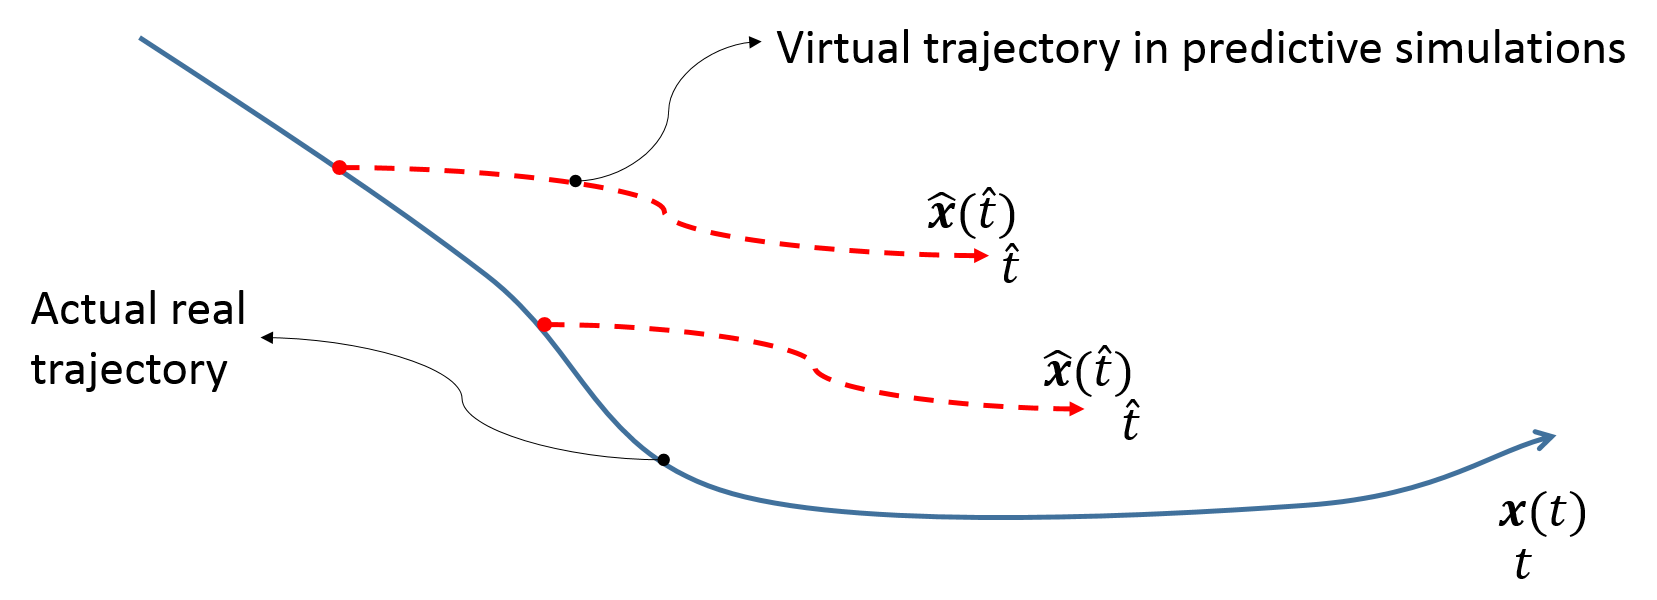
\includegraphics[width=0.8\textwidth]{rollouttrajs.png}
	\caption{Real trajectory and simulated virtual trajectory in the Rollout controller}
	\label{fig:rollouttrajs}
\end{figure}
%
The time derivative of the cost $J_k$, representing how much the computed cost change if the simulation is conducted $dt$ later in time, is given by:
%
\begin{align}
\dot{J}_k(t) = \frac{d}{dt} \int_{t}^{t+h}{  C_k \, d\hat{t} }
\end{align}
%
Using Leibniz's rule:
%
\begin{align}
\dot{J}_k(t) = C_k( t + h ) -  C_k( t ) +   \int_{t}^{t+h}{ \frac{\partial}{\partial t} C_k \, d\hat{t} }
\end{align}
%
for which it is possible to find an upper bound:
%
\begin{align}
\dot{J}_k(t) &\leq C_k^{max} -  0   +   \int_{t}^{t+h}{ \dot{C}_k^{max} \, d\hat{t} }  \\
\dot{J}_k(t) &\leq C_k^{max}  +   \dot{C}_k^{max} h
\end{align}
%
Note that compared to the last section analysis (fixed trajectory), there is an additional term  $\dot{C}_k^{max} h$ representing sensitivity of states trajectory in simulations. Then, most of the previous analysis is still valid, except that the bounds on cost variation of eq. \eqref{eq:costvariation}, are now given instead by:
%
\begin{align}
-\left[ C_k^{max}  +   \dot{C}_k^{max} h \right] \Delta t  \leq \Delta J_k \leq \left[ C_k^{max}  +   \dot{C}_k^{max} h \right] \Delta t
\label{eq:costvariationnew}
\end{align}
%
And the final result is modified to be:
%
\begin{align}
\Delta t \geq \frac{Q}{ C_k^{max}  +   \dot{C}_k^{max} h }
\end{align}
%

\subsubsection{Sensitivity of cost along simulated trajectories}
%
Regarding the new term, the time derivative of instantaneous cost in the simulation can be expressed as:
%
\begin{align}
\dot{C}_k    = \frac{\partial C_k}{\partial t} = \frac{\partial C_k}{\partial \vec{\tau}} \frac{\partial \vec{\tau}}{\partial \vec{\hat{x}}} \frac{\partial \vec{\hat{x}}}{\partial t} 
\end{align}
%
This term represent how much the computed cost can vary, between two simulations computed with $dt$ interval, for time interval shared by the two simulations. 

\paragraph{Cost function sensitivity}
%
The term $\frac{\partial C_k}{\partial \vec{\tau}}$ is the sensitivity of the used cost function with respect to computed torques. For a quadratic torque criterion $C_k = \vec{\tau}_k^T \vec{\tau}_k$, like always used in this thesis, it is equal to:
%
\begin{align}
\frac{\partial C_k}{\partial \vec{\tau}_k} = 2\vec{\tau}_k^T
\end{align}

\paragraph{Control law sensitivity}
%
The term $\frac{\partial \vec{\tau}}{\partial \vec{\hat{x}}}$ is a Jacobian matrix representing the sensitivity of computed torque with respect to states. This matrix could be computed analytically with the feedback laws, for the computed torque control law:
%
\begin{align}
\frac{\partial \vec{\tau}}{\partial \vec{\hat{x}}} = 
\left[ \begin{array}{c c}
	H_k^{-1} K_D & 0 \\ 0 & H_k^{-1} K_P
\end{array} \right] +
\left[ \begin{array}{c c}
	H_k^{-1} ( D + C + R_k^T B R_k ) & 0 \\ 0  & H_k^{-1} \frac{\partial \vec{g}}{\partial \vec{q}}
\end{array} \right] 
\end{align}
%
%
For the sliding mode control law, because of the additional discontinuous term $\vec{\tau}_d = G \sgn( \vec{s} )$, the derivative $\frac{\partial \vec{\tau}}{\partial \vec{\hat{x}}}$ can be unbounded when $s_i \approx 0$. However, the difference over a finite time interval $\Delta t$ is bounded since worst case scenario:
%
\begin{align}
-2G \leq \left[ \Delta \vec{\tau}_d \right]_i \leq 2G
\end{align}
%
Lets assume for simplicity that the cost function would penalize independently the continuous torque term and the discontinuous torque term:
%
\begin{align}
C_k = C_{c} + C_{d} = C_{c} + \vec{\tau}_d^T \vec{\tau}_d
\end{align}
%
then the resulting modified lower bound on minimum delay would be:
%
\begin{align}
\Delta t \geq \frac{Q - \operatornamewithlimits{max}\left[\vec{\tau}_d^T \vec{\tau}_d\right] h }{ C_{c}^{max}  +   \dot{C}_{c}^{max} h }
\end{align}
%
This shows that with large discontinuous gains, it would be harder to guarantee a minimum delay. There is thus a double advantages for using a smoothing technique (ex: boundary layer \cite{slotine_applied_1991} or higher order sliding mode \cite{perruquetti_sliding_2002}) for which the control law is not discontinuous. In addition to the advantage of smoothing the torque command, it would also make it easier to design a rollout gear selection that guarantee a minimum delay. Alternatively, as proposed in section \ref{sec:minimax}, reformulating the cost function to make it independent of the sign of $\vec{s}$ it another approach to alleviate this problem.  

\paragraph{Virtual trajectory sensitivity}
%
The term $\frac{\partial \vec{\hat{x}}}{\partial t}$ represents by how much the states at time $\hat{t}$ (in the simulation) would change if the simulation would have started $dt$ later. 
%
The virtual trajectory can be parametrized as the sum of the desired trajectory and errors:
%
\begin{align}
\vec{\hat{x}}( \hat{t} , t ) =  \vec{\hat{x}}_e( \hat{t} , t ) + \vec{\hat{x}}_d( \hat{t} )
\end{align}
%
Because the desired trajectory is independent of starting simulation time $t$, the sensitivity of the trajectory is only the sensitivity of this error term:
%
\begin{align}
\frac{\partial \vec{\hat{x}}}{\partial t}  = \frac{\partial \vec{\hat{x}}_e}{\partial t}
\end{align}
%
%
%%
%\begin{align}
%\vec{\hat{x}}_e( \hat{t} , t ) = \int_{t}^{t+h}{  \dot{\hat{\vec{x}}}_e \, d\hat{t} } + \vec{x}_e(t)
%\end{align}
%%
For the closed-loop system with the computed torque controller, the error dynamic is stable and linear, hence:
%
\begin{align}
\dot{\vec{x}}_e = A \vec{x}_e  \quad \Rightarrow \quad  \vec{x}_e( t ) = e^{A t} \vec{x}_e(t=0)
\end{align}
%
Similarly for the sliding mode controller, after all sliding surfaces are reached (happens in finite time) then the error dynamic is also linear and stable.
%
Using this matrix exponential solution for error trajectory in the simulations leads to 
%
\begin{align}
\vec{\hat{x}}_e( \hat{t} , t ) = e^{A (\hat{t} - t )} \vec{x}_e(t)  
\end{align}
%
since initial error in the simulations is the real error at time $t$. It is then possible to compute the sensitivity of virtual state trajectory with respect to simulation initialization time:
%
\begin{align}
\frac{\partial \vec{\hat{x}}}{\partial t}  = -A e^{A (\hat{t} - t )} \vec{x}_e(t) + e^{A (\hat{t} - t )} \dot{\vec{x}}_e(t) \leq \vec{b} \quad \forall \, \hat{t} > t
\end{align}
%
Hence trajectory sensitivity can thus be bounded, because the closed-loop error dynamic is linear and stable in simulations (matrix A only has eigenvalues with negative real parts).  

\paragraph{Sensitivity conclusions}
%
All in all, it is thus possible to conclude that:
\begin{enumerate}
	\item Sensitivity $\dot{C}_k$ is bounded (with a continuous control law)
	\item Sensitivity $\dot{C}_k \rightarrow 0$ far ahead in simulations as $\hat{t} \rightarrow \infty$
	\item Sensitivity $\dot{C}_k = 0$ if there is no tracking error ($ \vec{x}_e = \vec{0} \quad \dot{\vec{x}}_e = \vec{0}$)
\end{enumerate}
%
Note that conclusion 3 is consistent with the previous analysis (sec. \ref{sec:chat1}) where it was assumed a situation where all trajectories (real, desired and simulations) were all identical. Also conclusion 2 suggest that the sensitivity of future cost would no grow forever as the time horizon $h$ is increased, hence by using the following:
%
\begin{align}
\int_{t}^{t+h}{ \dot{C}_k \, d\hat{t} } \leq \dot{C}_k^{max} h
\end{align}
%
the result is probability very conservative and unadapted when the time horizon $h$ is very large.

